% Chapter 2: Background and Related Work

\section{Mapping Science as a Spatial Problem}

A map of science is always a map of a relation. Since the early work on visualizing knowledge domains, science mapping has turned relations among scientific objects into spatial form: papers, journals, authors, subject categories, research fronts, or disciplines become points, regions, and distances \parencite{borner2003visualizing}. The appeal of this tradition is clear. A map can summarize a large scientific system in a form that supports comparison, navigation, and interpretation. Its risk is equally clear: the apparent geometry depends on what relation has been mapped.

Classical bibliometric maps usually begin from relations such as citation, co-citation, bibliographic coupling, co-authorship, co-word occurrence, or journal/category assignment. Each relation answers a different question. Citation and co-citation structures capture intellectual and social traces left by published work. Bibliographic coupling emphasizes shared references. Co-word maps emphasize vocabulary. Category overlays position units inside an existing classification. Distance-based tools such as VOSviewer make this logic explicit by arranging objects so that spatial proximity reflects a chosen similarity structure \parencite{vaneck2010vosviewer}. Global overlay maps similarly show how research activity occupies predefined disciplinary regions \parencite{leydesdorff2013global}.

This thesis inherits the spatial logic of science mapping, but changes the object of measurement. It asks what happens when scientific fields are treated as distributions of documents in a dense representation space. In that setting, the relevant object is not only where a field is located, but how its papers occupy the surrounding space.

\section{From Bibliometric Relations to Semantic Representations}

Bibliometric relations are powerful because they encode collective scholarly behavior, but they are not identical to semantic proximity. Two papers may be close in citation space because they participate in the same research community, share a method, or inherit the same canonical references. They may be semantically close without citing one another, especially when similar problems emerge in different venues or disciplines. Conversely, category systems provide stable reference frames, but they impose boundaries before the analysis begins.

Text-based representations offer a complementary route. The vector-space tradition in information retrieval made documents comparable in a common numerical space \parencite{salton1983vector}. Later dense-vector models showed how semantic associations could be encoded in continuous coordinates \parencite{mikolov2013word2vec}. Such representations are useful here not because they reveal meaning without mediation, but because they make semantic proximity operational: every retained document has coordinates, and distances, neighborhoods, centroids, dispersion, and movement become measurable.

That move matters for science mapping. Instead of representing fields only through links among journals, references, or categories, a field can be represented through the distribution of its papers in semantic space. This does not make the representation more neutral than a citation network. Embeddings are model-defined geometries shaped by training data, language coverage, supervision objectives, and input text. Their value is that they expose a different layer of scientific structure: the language-based and citation-informed proximity of scientific documents.

\begin{figure}[H]
\centering
\caption[Citation topology and semantic geometry]{Citation topology and semantic geometry. The contrast is schematic: citation maps organize papers through observed links, whereas document embeddings make every retained paper comparable through coordinates, distances, and local density. This motivates the thesis shift from graph communities or category membership toward fields as distributions in semantic space.}
\label{fig:citation_semantic_contrast}
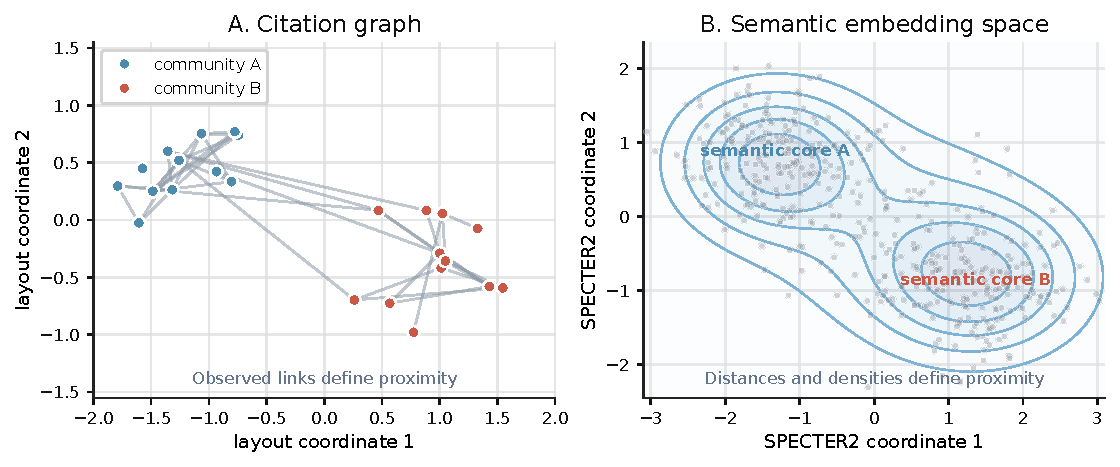
\includegraphics[width=\textwidth]{figures/fig_02_citation_semantic_contrast.pdf}
\end{figure}

The data source also matters. This thesis uses OpenAlex because it provides an open bibliographic infrastructure with works, concepts, venues, authors, institutions, and hierarchical research areas \parencite{priem2022openalex}. Open data makes the corpus auditable, but it does not remove coverage limits. Large bibliographic databases vary by field, document type, language, and metadata completeness \parencite{martinmartin2021google}, and recent comparisons document both the strengths of OpenAlex reference coverage and remaining metadata limitations \parencite{culbert2025reference}. For that reason, OpenAlex subfields are used as pragmatic analytical units, not as natural boundaries of science.

\section{Scientific Document Embeddings}

Scientific text is not generic text. Titles and abstracts contain specialized terminology, compressed argumentative structures, domain conventions, and technical phrases whose meaning depends on scientific context. Domain-adapted language models such as SciBERT were developed because scientific corpora differ systematically from general language corpora \parencite{beltagy2019scibert}. For this thesis, the relevant unit is not a word or sentence but a scientific work represented through its title and abstract.

SPECTER introduced document-level scientific embeddings learned with citation-informed supervision: papers that cite or are cited by one another provide a signal for document relatedness, so textual representation is trained with structural scholarly information \parencite{cohan2020specter}. SPECTER2 extends this line of work within the SciRepEval framework for evaluating scientific document representations across multiple task formats \parencite{singh2023scirepeval}. This makes SPECTER2 appropriate for a thesis that compares scientific works as documents rather than estimating word frequencies or topic mixtures.

The use of SPECTER2 does not mean that the embedding space is treated as ground truth. A 768-dimensional document vector is a compressed representation of title--abstract text under a particular model. It cannot capture the full methods, evidence, institutional context, or epistemic commitments of a paper. It can, however, provide a shared scientific document geometry in which sets of papers can be compared consistently. Chapter 4 explains the implemented representation pipeline; the role of the literature here is to justify why document-level scientific embeddings are a reasonable substrate for field-level morphology.

\section{From Semantic Location to Morphology}

Most uses of document embeddings begin with location: where is a paper, a topic, or a field in semantic space? Location is important, but it is incomplete. A centroid can summarize the average position of a field, yet it discards the field's internal spread, local packing, hub concentration, spectral structure, and temporal movement. The same field can be close in citation space, far in semantic location, and similar in morphology to another field. This thesis therefore shifts attention from where a field is located to how its papers occupy space around that location.

The idea has roots in earlier work on diversity, distance, and novelty. Stirling's diversity framework distinguishes variety, balance, and disparity, making clear that a collection cannot be characterized only by counting its elements \parencite{stirling2007diversity}. Work on cognitive distance similarly treats proximity and distance as conditions that shape learning and recombination \parencite{nooteboom2007cognitive}. Studies of scientific novelty show that unusual combinations can matter because they bridge distant regions of existing knowledge \parencite{uzzi2013atypical}. This thesis does not reproduce those measures directly. It adapts their intuition to dense semantic geometry: fields are distributions, and their shape can be measured.

Embedding-space morphology is the operational form of that idea. Dispersion describes how far papers spread around the field centroid. Local density describes how tightly papers pack into neighborhoods. Hubness describes whether a small subset of papers becomes disproportionately central in nearest-neighbor relations, a known phenomenon in high-dimensional spaces \parencite{radovanovic2010hubness}. Spectral structure summarizes how many principal directions are needed to describe variation. Temporal movement asks how those structures change across publication windows.

This geometric view requires caution. High-dimensional distances are affected by anisotropy, distance concentration, density variation, and hubness. Low-dimensional projections introduce a second layer of distortion. UMAP is a useful visualization method \parencite{mcinnes2018umap}, but nonlinear projections can change apparent distances, densities, and cluster shapes \parencite{chari2023specious,wattenberg2016tsne}. For that reason, this thesis uses PCA, PCoA, and UMAP only for communication and exploratory display. Quantitative morphology is computed in the original SPECTER2 embedding space.

\section{Positioning of This Thesis}

The gap addressed by this thesis lies between science mapping and scientific document representation. Existing science maps often emphasize bibliometric topology, classification overlays, topic structure, or two-dimensional visualization. Scientific document embeddings make a shared semantic geometry available, but they are often used to cluster papers, retrieve similar documents, or draw maps. Here the geometry is used differently: to measure field-level morphology.

The contribution is a disciplined separation of location, shape, trajectory, and taxonomy. Semantic location refers to where a subfield's centroid sits in embedding space. Static morphology describes the full-period shape of the subfield's paper distribution. Temporal trajectories describe how morphology changes across windows. Morphological similarity compares fields or subfields through profile distances. Clustering compresses those profiles into typological anchors, while remaining exploratory rather than taxonomic. This caution is important because no clustering procedure provides a uniquely objective partition of a data space \parencite{kleinberg2002clustering}.

This positioning narrows the claim. The thesis is not a topic model, a citation-network clustering project, a paper-level community detection study, a productivity or impact analysis, a UMAP-based map, or a replacement for OpenAlex taxonomy. Those approaches answer different questions. The present framework asks how field-level paper distributions are shaped in a shared scientific document geometry.

The following chapters make that question operational. Chapter 3 defines the OpenAlex corpus and the subfield as the analytical unit. Chapter 4 defines the SPECTER2 representation and the separation between measurement space and visualization. Chapter 5 develops the embedding-space morphology metrics. Chapters 6 to 9 then use those metrics to compare static morphology, temporal trajectories, morphological similarity, and exploratory typological structure.
